\documentclass[11pt]{article}
%\usepackage{fullpage,graphicx,algorithm,algorithmic,bm,amsmath,amsthm,amssymb,color,hyperref,cite,natbib}

% if you need to pass options to natbib, use, e.g.:
%\PassOptionsToPackage{numbers}{natbib}
\usepackage{natbib,fullpage}
\usepackage{bm,amsmath,amsthm,amssymb,multicol,algorithmic,algorithm,enumitem}
\usepackage{color,wrapfig}
\usepackage[textwidth=1cm,textsize=footnotesize]{todonotes}
% ready for submission
\usepackage{neurips_2020}

\usepackage{lipsum}
\usepackage[colorlinks=true,
linkcolor=red,
urlcolor=blue,
citecolor=blue]{hyperref}

\usepackage{xargs}
\usepackage{stmaryrd}

\setlength{\parskip}{.2cm}

\newtheorem{Fact}{Fact}
\newtheorem{Lemma}{Lemma}
\newtheorem{Prop}{Proposition}
\newtheorem{Theorem}{Theorem}
\newtheorem{Def}{Definition}
\newtheorem{Corollary}{Corollary}
\newtheorem{Conjecture}{Conjecture}
\newtheorem{Property}{Property}
\newtheorem{Observation}{Observation}
%\theorembodyfont{\rmfamily}
\newtheorem{Exa}{Example}
\newtheorem{assumption}{H\!\!}
\newtheorem{assumptionA}{G\!\!}
\newtheorem{Remark}{Remark}
\newtheorem*{Lemma*}{Lemma}
\newtheorem*{Theorem*}{Theorem}
 \makeatletter
\renewenvironment{proof}[1][\proofname]{%
   \par\pushQED{\qed}\normalfont%
   \topsep6\p@\@plus6\p@\relax
   \trivlist\item[\hskip\labelsep\bfseries#1]%
   \ignorespaces
}{%
   \popQED\endtrivlist\@endpefalse
}
\makeatother
\usepackage{shortcuts_OPT}

%\renewcommand{\textwidth}{5.5in}

% Here's the definition of Sb, stolen from amstex
    \makeatletter
    \def\multilimits@{\bgroup
  \Let@
  \restore@math@cr
  \default@tag
 \baselineskip\fontdimen10 \scriptfont\tw@
 \advance\baselineskip\fontdimen12 \scriptfont\tw@
 \lineskip\thr@@\fontdimen8 \scriptfont\thr@@
 \lineskiplimit\lineskip
 \vbox\bgroup\ialign\bgroup\hfil$\m@th\scriptstyle{##}$\hfil\crcr}
    \def\Sb{_\multilimits@}
    \def\endSb{\crcr\egroup\egroup\egroup}
\makeatother

\newtheoremstyle{t}         %name
    {\baselineskip}{2\topsep}      %space above and below
    {\rm}                   %Body font
    {0pt}{\bfseries}  %Heading indent and font
    {}                      %after heading
    { }                      %head after space
    {\thmname{#1}\thmnumber{#2}.}

\theoremstyle{t}
\newtheorem{q}{Q}
\parindent=0pt

\makeatletter
\DeclareRobustCommand*\cal{\@fontswitch\relax\mathcal}
\makeatother

\newcommand{\tcr}[1]{\textcolor{red}{#1}}
\newcommand{\mathbbm}[1]{\text{\usefont{U}{bbm}{m}{n}#1}}

\begin{document}
\title{Fast Two-Time-Scale Noisy EM Algorithms}
\author{
  Belhal Karimi \\
  Cognitive And Computing Lab\\
  Baidu Research\\
  Beijing, China \\
  \texttt{belhal.karimi@baidu.com} 
   \And
  Ping Li \\
  Cognitive And Computing Lab\\
  Baidu Research\\
  Beijing, China \\
  \texttt{liping@baidu.com} }
\date{\today}

\maketitle

\begin{abstract}
Training latent data models using the EM algorithm is the most common choice for current learning tasks. 
Variants of the EM to scale to large datasets and bypass the impossible conditional expectation of the latent data for most nonlinear models have been initially introduced respectively by \citep{neal1998view}, using incremental updates, and \citep{wei1990monte, delyon1999}, using Monte-Carlo (MC) approximations.
In this paper, we propose to combine those both techniques in a single class of methods called Two-Time-Scale EM Methods. 
We motivate the choice of a double dynamics by invoking the variance reduction virtue of each stage of the method on both noise: the incremental update and the MC approximation.
We establish finite-time convergence bounds for nonconvex objective function and independent of the initialization.
Numerical applications are also presented in this article to illustrate our findings.
\end{abstract}


\section{Introduction}
Learning latent data models is critical for modern machine learning problems, see \citep{mclachlan2007algorithm} for references.
We formulate the training of such model as the following empirical risk minimization problem:
\beq \label{eq:em_motivate}
\min_{ \param \in \Param }~ \overline{\calL} ( \param ) \eqdef \Pen (\param) + \calL ( \param )~~\text{with}~~\calL ( \param ) = \frac{1}{n} \sum_{i=1}^n \calL_i( \param) \eqdef  \frac{1}{n} \sum_{i=1}^n \big\{ - \log g( y_i ; \param ) \big\}\eqs,
\eeq
We denote the observations by $\{y_i\}_{i=1}^n$, $\Param \subset \rset^d$ is the convex parameters space.
We consider a regularized model where $\Pen : \Param \rightarrow \rset$ is a smooth convex regularization function and for $\param \in \Param$, $g(y;\param)$ is the (incomplete) likelihood of each individual  observation.
The objective function $ \overline{\calL} ( \param )$ is possibly \emph{nonconvex} and is assumed to be lower bounded $ \overline{\calL} ( \param ) > - \infty$ for all $\param \in \Param$.

%We assume that $ \overline{\calL} ( \param ) > - \infty$ for all $\param \in \Param$.
In the latent variable model,  $g(y_i ; \param)$, is the marginal of the
complete data likelihood defined as $f(z_i,y_i; \param)$, i.e. $g(y_i; \param) = \int_{\Zset} f (z_i,y_i;\param) \mu(\rmd z_i)$, where $\{ z_i \}_{i=1}^n$ are the (unobserved)
latent variables.   
In this papaer, we make the assumption of a complete model belonging to the curved exponential family, \ie
\beq \label{eq:exp}
f(z_i,y_i; \param) = h  (z_i,y_i) \exp \big( \pscal{S(z_i,y_i)}{\phi(\param)} - \psi(\param) \big)\eqs,
\eeq
where $\psi(\param)$, $h(z_i,y_i)$ are scalar functions, $\phi(\param) \in \rset^k$ is a vector function, and $S(z_i,y_i) \in \rset^k$ is the complete data sufficient statistics.

Full batch EM \citep{dempster1977Maximum} is the method of reference for that kind of task and is a two steps procedure. The {\sf E-step} amounts to computing the conditional expectation of the complete data sufficient statistics, 
\begin{equation}
\label{eq:definition-overline-bss}
\overline{\bss}(\param)= \frac{1}{n} \sum_{i=1}^n \overline{\bss}_i(\param) \quad  \text{where}  \quad \overline{\bss}_i(\param)= \int_{\Zset} S(z_i,y_i) p(z_i|y_i;\param) \mu(\rmd z_i) \,.
\end{equation}
The {\sf M-step} is given by
\beq \label{eq:mstep}
\textsf{M-step:}~~\hat{\param} = \overline{\param}( \overline{\bss}(\param) ) \eqdef \argmin_{ \vartheta \in \Param } ~\big\{ \Pen( \vartheta ) + \psi( \vartheta) - \pscal{ \overline{\bss}(\param)}{ \phi ( \vartheta) } \big\},
\eeq

Two caveats of this method are the following: (a) with the explosion of data, the first step of the EM is computationally inefficient as it requires a full pass over the dataset at each iteration and (b) the complexity of modern models makes the expectation intractable. So far, both challenges have been addressed separately, to the best of our knowledge, and we give an overview of current solutions in the sequel.

\paragraph{Prior Work} Inspired by stochastic optimization procedures, \citep{neal1998view} and \citep{cappe2009line} developed respectively an incremental and an online variant of the \textsf{E-step} in models where the expectation is computable then extensively used and studied in \citep{nguyen2020mini, liang2009online,cappe2011online}.
Some improvements of that methods have been provided and analyzed, globally and in finite-time, in \citep{karimi2019global} where variance reduction techniques taken from the optimization literature have been efficiently applied to scale the EM algorithm to large datasets.

Regarding the computation of the expectation under the posterior distribution, the first method was the Monte-Carlo EM (MCEM) introduced in the seminal paper \citep{wei1990monte} where a MC approximation fo this expectation is computed. A variant of that method is the Stochastic Approximation of the EM (SAEM) in \citep{delyon1999} leveraging the power of Robbins-Monro type of update \citep{robbins1951stochastic} to ensure pointwise convergence of the vector of estimated parameters rather using a decreasing stepsize than increasing the number of MC samples.
The MCEM and the SAEM have been successfully applied in mixed effects models \citep{mcculloch1997maximum,hughes1999mixed,baey2016nonlinear} or to do inference for joint modelling of time to event data coming from clinical trials in \citep{das2010Inferences}, among other applications.

Recently, an incremental variant of the SAEM was proposed in \citep{kuhn2019properties} showing positive empirical results but its analysis is limited to asymptotic consideration. 
Gradient-based methods have been developed and analyzed in \citep{zhu2017high} but they remain out of the scope of this paper as they tackle the high-dimensionality issue.


\paragraph{Contributions} This paper \textit{introduces} and \textit{analyzes} a new class of methods which purpose is to combine both solutions proposed in the past years in a two-time-scale manner in order to optimize \eqref{eq:em_motivate} for current modern examples and settings. The main contributions of the paper are:
\begin{itemize}

\item We propose a two-time-scale method based on Stochastic Approximation (SA), to alleviate the problem of MC computation, and on Incremental updates, to scale to large datasets. We describe in details the edges of each level of our method based on variance reduction arguments. The derivation of such class of algorithms has two advantages. First, it combines two powerful ideas, commonly used separately, to tackle large scale and highly nonlinear learning tasks. Then, it gives a simple formulation as a \textit{scaled-gradient method}, as introduced in \citep{karimi2019global}, which makes the global analysis accessible.

\item We also establish global (independent of the initialization) and finite-time (true at each iteration) upper bounds on a classical suboptimality condition in the nonconvex literature, \ie\ the second order moment of the gradient of the objective function. 


\end{itemize}

In Section~\ref{sec:tts} we give rigorous mathematical definitions of the various updates used for both incremental and Monte-Carlo EMs and we introduce the main class of new algorithms, based on two different dynamics, we are proposing to analyze and compare to baselines algorithms. Section~\ref{sec:mainanalysis} presents the main theoretical guarantees of this newly introduced two-time-scale class of algorithms. Results are given both in finite-time and in the nonconvex setting.
Finally, we illustrate the advantages of our method in Section~\ref{sec:numerical} on two numerical experiments.



\section{Two-Time-Scale Stochastic EM Algorithms}\label{sec:tts}
We recall and formalize in this section the different methods found in the literature that aim to solving the large scale problem and the intractable expectation. 
We then provide the general framework of our method to efficiently tackle the optimization problem \eqref{eq:em_motivate}.
\subsection{Monte Carlo Integration and Stochastic Approximation} \label{sec:sEM}
As mentioned in the introduction, for complex and possibly nonlinear models, the expectation under the posterior distribution defined in \eqref{eq:definition-overline-bss} is not tractable. In that case, the first solution involves computing a Monte Carlo integration of that latter term. 
For all $ i \in \inter$, draw for $m \in \llbracket 1, M \rrbracket$, samples $z_{i,m} \sim p(z_i|y_i;\theta)$ and compute the MC integration $\tilde{\bss}$ of the deterministic quantity $\overline{\bss}(\param)$:
\beq\label{eq:mcstep}
\textsf{MC-step}:~ \tilde{\bss} = \frac{1}{n} \sum_{i=1}^n\frac{1}{M} \sum_{m=1}^M S(z_{i,m}, y_i)
\eeq
and compute $\hat{\param} = \overline{\param}( \hat{\bss} ) $.

This algorithm bypasses the intractable expectation issue but is rather computationally expensive in order to reach point wise convergence ($M$ needs to be large).

As a result, an alternative to that stochastic algorithm is to use a Robbins-Monro (RM) type of update.
We denote
\beq\label{eq:stats}
\tilde{S}^{(k+1)} = \frac{1}{n} \sum_{i=1}^n \tilde{S}^{(k+1)}_i = \frac{1}{n} \sum_{i=1}^n\frac{1}{M} \sum_{m=1}^M S(z_{i,m}^{(k)}, y_i)
\eeq
where $z_{i,m}^{(k)} \sim p(z_i|y_i;\theta^{(k)})$.
At iteration $k$, the sufficient statistics $\hat{\bss}^{(k+1)}$ is approximated as follows:

\beq\label{eq:rmstep}
\textsf{SA-step}:~ \hat{\bss}^{(k+1)} =  \hat{\bss}^{(k)}  + \gamma_{k+1}(\tilde{S}^{(k+1)} - \hat{\bss}^{(k)} )
\eeq

where $\{ \gamma_{k} \}_{k=1}^\infty \in [0,1]$ is a sequence of decreasing step sizes to ensure asymptotic convergence.
This is called the Stochastic Approximation of the EM (SAEM), see \citep{delyon1999} and allows a smooth convergence to the target parameter.
It represents the \textit{first level} of our algorithm (needed to temper the variance and noise implied by MC integration).

In the next section, we derive variants of this algorithm to adapt of the sheer size of data of today's applications.

\subsection{Incremental and Bi-Level Inexact EM Methods} \label{sec:sEM}
Strategies to scale to large datasets include classical incremental and variance reduced variants.
We will explicit a general update that will cover those variants and that represents the \textit{second level} of our algorithm, namely the incremental update of the noisy statistics $\hat{S}^{(k)}$ inside the RM type of update.

\beq \label{eq:sestep}
\textsf{Inexact-step}:~\tilde{S}^{(k+1)} = \tilde{S}^{(k)} + \rho_{k+1} \big( \StocEstep^{(k+1)}- \tilde{S}^{(k)}  \big),
\eeq

Note $\{ \rho_{k} \}_{k=1}^\infty \in [0,1]$ is a sequence of step sizes, $\StocEstep^{(k)}$ is a proxy for $\tilde{S}^{(k)}$,
If the stepsize is equal to one and the proxy $\StocEstep^{(k)} = \hat{S}^{(k)}$, i.e., computed in a full batch manner as in \eqref{eq:stats}, then we recover the SAEM algorithm.
Also if $\rho_{k}=1$, $\gamma_{k}=1$ and $\StocEstep^{(k)} = \tilde{S}^{(k)}$, then we recover the Monte Carlo EM algorithm.

We now introduce three variants of the SAEM update depending on different definitions of the proxy $\StocEstep^{(k)}$ and the choice of the stepsize $\rho_k$.
Let $i_k \in \inter$ be a random index drawn at iteration $k$ and $\tau_i^k = \max \{ k' : i_{k'} = i,~k' < k \}$ be the iteration index where $i \in \inter$ is last drawn prior to iteration $k$.
For iteration $k \geq 0$, the \FISAEM\ method draws \emph{two} indices \emph{independently} and uniformly as $i_k, j_k \in \inter$. In addition to $\tau_i^k$ which was defined \wrt $i_k$, we define $t_j^k = \{ k' : j_{k'} = j , k' < k \}$ to be the iteration index where the sample $j \in \inter$ is last drawn as $j_k$ prior to iteration $k$. With the initialization $\overline{\StocEstep}^{(0)} = \overline{\bss}^{(0)}$, we use a slightly different update rule from SAGA inspired by \citep{reddi2016fast}. Then, we obtain:
\begin{align}
&\emph{(\ISAEM\ \citep{karimi2019non, kuhn2019properties})} & \StocEstep^{(k+1)} &= \StocEstep^{(k)} + {\textstyle \frac{1}{n}}\big( \tilde{S}_{i_k}^{(k)}  - \tilde{S}_{i_k}^{(\tau_{i_k}^k)} \big) \label{eq:isaem} \\
&\emph{(\SAEMVR\ This paper )} &\StocEstep^{(k+1)} &= \tilde{S}^{(\ell(k))} +  \big( \tilde{S}_{i_k}^{(k)}  -\tilde{S}_{i_k}^{(\ell(k))}   \big) \label{eq:vrsaem}\\
&\emph{(\FISAEM\ This paper )} &\StocEstep^{(k+1)} &= \overline{\StocEstep}^{(k)} + \big( \tilde{S}_{i_k}^{(k)}  - \tilde{S}_{i_k}^{(t_{i_k}^k)} \big) \label{eq:fisaem}\\
&    &\overline{\StocEstep}^{(k+1)} &= \overline{\StocEstep}^{(k)} + n^{-1} \big( \tilde{S}_{j_k}^{(k)}  - \tilde{S}_{j_k}^{(t_{j_k}^k)} \big).
%\emph{(SAGA-EM)} & ~~~~\StocEstep^{(k+1)} = s & \gamma_{k+1} =
\end{align}
The stepsize is set to $\rho_{k+1} = 1$ for the \ISAEM\ method; $\rho_{k+1} = \gamma$ is  constant for the \SAEMVR\ and \FISAEM\ methods.
Moreover, for \ISAEM\ we initialize with $\StocEstep^{(0)} = \tilde{S}^{(0)}$; for \SAEMVR\, we set an epoch size of $m$ and define $\ell(k) \eqdef m \lfloor k/m \rfloor$ as the first iteration number in the epoch that iteration $k$ is in. \vspace{-.2cm}


\subsection{Two-Time-Scale Noisy EM methods}
We now introduce the general method derived using the two variance reduction techniques described above.
Algorithm~\ref{alg:ttsem} leverages both levels \eqref{eq:rmstep} and \eqref{eq:sestep} in order to output a vector of fitted parameters $\hat{\param}^{(K)}$ where $K$ is some randomly chosen termination point.

The updates in \eqref{eq:twolevels} is said to have two timescales as the step sizes satisfy $\lim \limits_{k \to \infty} \gamma_k/\rho_k < 1$ such that $ \tilde{S}^{(k+1)} $  is updated at a faster timescale than $\hat{\bss}^{(k+1)}$.

\begin{algorithm}[H]
\caption{Two-Time-Scale Noisy EM methods.}\label{alg:ttsem}
  \begin{algorithmic}[1]
  \STATE \textbf{Input:} initializations $\hat{\param}^{(0)} \leftarrow 0$, $\hat{\bss}^{(0)} \leftarrow \hat{S}^{(0)}$, $K_{\sf max}$ $\leftarrow$ max.~iteration number. \STATE Set the terminating iteration number, $K \in \{0,\dots,K_{\sf max}-1\}$, as a discrete r.v.~with:\vspace{-.1cm}
  \beq \label{eq:random}
   P( K = k ) = \frac{ \gamma_{k} }{\sum_{\ell=0}^{K_{\sf max}-1} \gamma_\ell}.\vspace{-.2cm}
  \eeq
  \FOR {$k=0,1,2,\dots, K$}
  \STATE Draw index $i_k \in \inter$ uniformly (and $j_k \in \inter$ for \FISAEM).
     \STATE Compute $\hat{S}_{i_k}^{(k)}$ using the {\sf MC-step} \eqref{eq:mcstep},  for the drawn indices.
   \STATE Compute the surrogate sufficient statistics $\StocEstep^{(k+1)}$ using \eqref{eq:isaem} or \eqref{eq:vrsaem} or \eqref{eq:fisaem}.
   \STATE Compute $\hat{S}^{(k+1)}$ and $\hat{\bss}^{(k+1)}$ using respectively \eqref{eq:sestep} and \eqref{eq:rmstep}:
\beq \label{eq:twolevels}
\begin{split}
& \tilde{S}^{(k+1)} = \tilde{S}^{(k)} + \rho_{k+1} \big( \StocEstep^{(k+1)}- \tilde{S}^{(k)}  \big)\\
&  \hat{\bss}^{(k+1)} =  \hat{\bss}^{(k)}  + \gamma_{k+1}(\tilde{S}^{(k+1)} - \hat{\bss}^{(k)} )
\end{split}
\eeq
   \STATE Compute $\hat{\param}^{(k+1)}$ via the {\sf M-step} \eqref{eq:mstep}.
\ENDFOR
\STATE \textbf{Return}: $\hat{\param}^{(K)}$.
%\STATE \textbf{Return:} $\prm_t$.
  \end{algorithmic}
\end{algorithm}



\section{Global and Finite Time Analysis of the Scheme} \label{sec:mainanalysis}
First, we consider the following minimization problem on the statistics space:
\beq\label{eq:em_sspace}
\min_{ {\bss} \in \Sset }~  V ( {\bss} ) \eqdef \overline\calL( \op(\bss) ) = \Pen (  \op(\bss) ) + \frac{1}{n} \sum_{i=1}^n {\cal L}_i (  \op(\bss) )
\eeq
It has been shown that this minimization problem is equivalent to the optimization problem \eqref{eq:em_motivate}, see \citep[Lemma2]{karimi2019global}

\begin{assumption}\label{ass:convset}
$\Theta$ is an open set of $\rset^d$ and the sets $\Zset, \Sset$ are measurable open sets such that:
\beq
\Sset \supset \left\{  n^{-1} \sum_{i=1}^n u_i, u_i \in {\rm conv}(\overline{\bss}_i(\param))  \right\}
\eeq
where $\overline{\bss}_i(\param)$ is defined in \eqref{eq:definition-overline-bss}.
\end{assumption}

\begin{assumption}\label{ass:expected}
The conditional distribution is smooth on ${\rm int}(\Param)$. For any $i \in \inter$, $z \in \Zset$, $\param, \param' \in {\rm int} (\Param)^2$, we have
$\big| p( z | y_i; \param ) - p( z | y_i; \param' ) \big| \leq  \Lip{p} \| \param - \param' \|$.
%For any $i \in \inter$, the map $\param \to \overline{\bss}_i(\param)$ is continuously differentiable in $\param$.
\end{assumption}

We also recall from the introduction that we consider curved exponential family models. besides:
\begin{assumption} \label{ass:reg}
For any $\bm{s} \in \Sset$, the function $\param \mapsto L(s,\param) \eqdef \Pen( \param ) + \psi( \param) - \pscal{ \bss}{ \phi ( \param) }$ admits a unique global minimum $\mstep{\bss} \in {\rm int}(\Param)$.
In addition, $\jacob{\phi}{\param}{\overline{\param}(\bss )}$ is full rank and $\overline{\param}( \bss )$ is $\Lip{\theta}$-Lipschitz.
\end{assumption}
Similar to \citep{karimi2019global}, we denote by $\hess{L}{\param}(\bss,\param)$ the Hessian (w.r.t to $\param$ for a given value of $\bss$) of the function $\param \mapsto L(\bss,\param)= \Pen(\param) + \psi(\param) -\pscal{\bss}{\phi(\param)}$, and define
\beq\label{eq:Bss}
\operatorname{B}( \bss ) \eqdef\jacob{ \phi }{ \param }{ \mstep{\bss} } \Big( \hess{L}{\param}( {\bss},  \mstep{\bss} )  \Big)^{-1} \jacob{ \phi }{ \param }{ \mstep{\bss} }^\top.
\eeq
\begin{assumption}\label{ass:eigen}
It holds that $ \upsilon_{\max} \eqdef \sup_{\bss \in \Sset} \| \operatorname{B}( \bss ) \| < \infty$ and $0 < \upsilon_{\min}  \eqdef \inf_{\bss \in \Sset} \lambda_{\rm min} ( \operatorname{B}( \bss ) )$.
There exists a constant $\Lip{B}$ such that for all $\bss, \bss' \in \Sset^2$, we have $ \| \operatorname{B}( \bss ) - \operatorname{B}( \bss' )  \| \leq \Lip{B} \| {\bss} - {\bss}' \|$.
\end{assumption}

We now formulate the main difference with the work done in \citep{karimi2019global}. 
The class of algorithms we develop in this paper are two time-scale where the first stage corresponds to the variance reduction trick used in \citep{karimi2019global} in order to accelerate incremental methods and kill the variance induced by the index sampling. 
The second stage is the Robbins-Monro type of update that aims to kill the variance induced by the MC approximations

Indeed the expectations \eqref{eq:definition-overline-bss} are never available and requires Monte Carlo approximation.
Thus, at iteration $k+1$, we introduce the errors when approximating the quantity $ \overline{\bss}_i(\hat{\param}(\hat{\bss}^{(k-1)}))$.
For all $i \in \inter$, $r > 0$ and $\vartheta \in \Theta$, define:
\beq\label{eq:mcerror}
\eta_{i}^{(r)} \eqdef \tilde{S}_{i}^{(r)} -  \overline{\bss}_i(\vartheta^{(r)})
\eeq

For instance, we consider that the MC approximation is unbiased if for all $ i \in \inter$ and $m \in \llbracket 1, M \rrbracket$, the samples $z_{i,m} \sim p(z_i|y_i;\theta)$ are i.i.d. under the posterior distribution, \ie $\EE[\eta_{i}^{(r)}|{\cal F}_r] = 0$ where  ${\cal F}_r$ is the filtration up to iteration $r$.

The following results are derived under the assumption of control of the fluctuations implied by the approximation stated as follows:
\begin{assumption}\label{ass:mcerror}
There exist a positive sequence of MC batch size $\{M_r\}_{r > 0}$ and constants $(C, C_{\eta})$ such that for all $k >0$, $i \in \inter$ and $\vartheta \in \Theta$:
\beq\label{eq:boundederror}
\EE\left[\norm{\eta_{i}^{(r)}}^2 \right] \leq \frac{C_{\eta}}{M_r} \quad \textrm{and} \quad \EE\left[\norm{\EE[\eta_{i}^{(r)}|{\cal F}_r]}^2\right] \leq \frac{C}{M_r}
\eeq
\end{assumption}


In that setting, we can prove two important results on the Lyapunov function. The first one suggests smoothness:
\begin{Lemma} \label{lem:smooth}
\citep{karimi2019global} Assume H\ref{ass:expected}, H\ref{ass:reg}, H\ref{ass:eigen}.  
For all $\bss,\bss' \in \Sset$ and $i \in \inter$, we have
\beq \label{eq:smooth}
\| \overline{\bss}_i ( \overline{\param} ({\bss})) - \overline{\bss}_i ( \overline{\param} ({\bss}' )) \| \leq \Lip{{\bss}} \| {\bss} - {\bss}' \|,~~\| \grd  V ( {\bss} ) - \grd  V ( {\bss}' ) \| \leq \Lip{V} \| {\bss} - {\bss}' \|,
\eeq
where $\Lip{\bss} \eqdef C_{\Zset} \Lip{p} \Lip{\theta}$ and $\Lip{V}  \eqdef \upsilon_{\max} \big( 1 + \Lip{{\bss}} \big) + \Lip{B} C_{\Sset}$.
\end{Lemma}
and the second one suggests a growth condition on the gradient of $V$ depending on the mean field of the algorithm:
\begin{Lemma}\label{lem:growth}
Assume H\ref{ass:reg},H\ref{ass:eigen}. For all $\bss \in \Sset$,
\beq \label{eq:semigrad}
\upsilon_{\min}^{-1} \pscal{\grd V ( {\bss} ) }{ {\bss} - \os( \op ({\bss})) }
\geq \big\| {\bss} - \os( \op ({\bss})) \big\|^2 \geq \upsilon_{\max}^{-2} \| \grd V ( {\bss} ) \|^2,
\eeq
\end{Lemma}
See proofs of this Lemma in Appendix~\ref{app:growth}.

\subsection{Global Convergence of Incremental Noisy EM Algorithms}
Following the asymptotic analysis of update \eqref{eq:isaem}, we present a finite-time analysis of the incremental variant of the Stochastic Approximation of the EM algorithm.

The first intermediate result is the computation of the quantity $\hat{S}^{(k+1)} - \hat{\bss}^{(k)}$, which corresponds to the dirft term of \eqref{eq:rmstep} and reads as follows:
\begin{Lemma} \label{lem:meanfield_isaem}
 Assume H\ref{ass:convset}. The update \eqref{eq:isaem} is equivalent to the following update on the resulting statistics 
\beq
\hat{\bss}^{(k+1)} =  \hat{\bss}^{(k)}  + \gamma_{k+1} \big( \tilde{S}^{(k+1)} - \hat{\bss}^{(k)} \big)
\eeq 
Also:
\beq
\EE\left[\tilde{S}^{(k+1)} - \hat{\bss}^{(k)}\right] = \EE\left[\overline{\bss}^{(k)} - \hat{\bss}^{(k)}\right] + \left(1 - \frac{1}{n} \right) \EE\left[\frac{1}{n} \sum_{i=1}^n \tilde{S}_i^{(\tau_i^k)}- \hat{\bss}^{(k)}\right]  +\frac{1}{n}\EE\left[\eta_{i_k}^{(k+1)}\right]
\eeq
where $\overline{\bss}^{(k)}$ is defined by \eqref{eq:definition-overline-bss} and $\tau_i^k = \max \{ k' : i_{k'} = i,~k' < k \}$.
\end{Lemma}

The following main result for the \ISAEM\ algorithm is derived under a control of the Monte Carlo fluctuations as described by assumption H~\ref{ass:mcerror}.
Typically, the controls exhibited below are of interest when the number of MC samples $M_k$ increase with the iteration index $f$.

\begin{Theorem}\label{thm:isaem}
Let $K_{\max }$ be a positive integer. 
Let $\left\{\gamma_{k}, k \in \mathbb{N}\right\}$ be a sequence of positive step sizes and consider the \ISAEM\ sequence $\left\{\hat{\bss}^{(k)}, k \in \mathbb{N}\right\}$ obtained with $\rho_{k+1}=1$ for any $k > 0$.

Assume that $ \hat{\bss}^{(k)} \in \mathcal{S}$ for any $k \leq K_{\max }$.

\textcolor{red}{TO COMPLETE WITH BOUND}

\end{Theorem} 
See proof in Appendix~\ref{app:theoremisaem}.
%Assume that $\widehat{S}^{k} \in \mathcal{S}$ for any $k \leq K_{\max }$ Let $\nu, \bar{\nu} \in\{0,1\}$ with the convention $\nu=0$ iff the approximations are unbiased, and $\bar{\nu}=0$ iff for any $k \geq 0,\left\|\eta_{k+1}^{(1)}\right\|=\left\|\eta_{k+1}^{(2)}\right\|=\varepsilon^{(0)}=0$
%For any positive numbers $\beta_{1}, \cdots, \beta_{K_{\max }-1}$ and $\beta_{0} \in\left(0, v_{\min } / v_{\max }^{2}\right),$ it holds
%$\sum_{k=0}^{K_{\max }-1} \alpha_{k} \mathbb{E}\left[\left\|\bar{s} \circ \operatorname{T}\left(\widehat{S}^{k}\right)-\widehat{S}^{k}\right\|^{2}\right]+\sum_{k=0}^{K_{\max }-1} \delta_{k} \mathbb{E}\left[\left\|\frac{1}{n} \sum_{i=1}^{n} \widetilde{S}_{k+1, i}-\bar{s} \circ \top\left(\widehat{S}^{k}\right)\right\|^{2}\right]$
%$\leq \mathbb{E}\left[V\left(\widehat{S}^{0}\right)\right]-\mathbb{E}\left[V\left(\widehat{S}^{K_{\max }}\right)\right]$
%$+\xi_{0}\left(K_{\max }, n\right) \mathbb{E}\left[\varepsilon^{(0)}\right]+\bar{\nu} \Xi_{1}\left(\eta^{(1)}, K_{\max }, n\right)+\bar{\nu} \Xi_{2}\left(\eta^{(2)}, K_{\max }, n\right)$
%for any $k=0, \ldots, K_{\max }-1$
%$\alpha_{k} \stackrel{\text { def }}{=} \gamma_{k+1}\left(v_{\min }-\nu v_{\max }^{2} \beta_{0}-(1+\nu) \frac{L_{\dot{V}}}{2} \gamma_{k+1}\left\{1+(1+\bar{\nu})(1+\nu) L^{2} \Lambda_{k}\right\}\right)$
%$\delta_{k} \stackrel{\text { def }}{=}(1+\nu) \frac{L_{\dot{V}}}{2} \gamma_{k+1}^{2}\left(1+(1+\bar{\nu})(1+\nu) \frac{\Lambda_{k}}{\left(1+\beta_{k+1}^{-1}\right)}\right)$
%with $\Lambda_{K_{\max }-1}=0$ and for $k=0, \ldots, K_{\max }-2$
%$\Lambda_{k} \stackrel{\text { def }}{=}\left(1+\frac{1}{\beta_{k+1}}\right) \sum_{j=k+1}^{K_{\max }-1} \gamma_{j+1}^{2} \prod_{\ell=k+2}^{j}\left(1-\frac{1}{n}+\beta_{\ell}+(1+\bar{\nu})(1+\nu) L^{2} \gamma_{\ell}^{2}\right)$
%$\xi_{0}, \Xi_{1}$ and $\Xi_{2}$ are non negative real numbers; their explicit expressions can be found in Section $4.6,$ Eqs $(54),(55)$ and $(56) .$ By convention, $\prod_{\ell \in \emptyset} a_{\ell}=1$

\subsection{Global Convergence of Two-Time-Scale Noisy EM Algorithms}
We now proceed by giving our main result regarding the global convergence of the \FISAEM\ algorithm.

\begin{Theorem}\label{thm:fisaem}
Let $K_{\max }$ be a positive integer. 
Let $\left\{\gamma_{k}, k \in \mathbb{N}\right\}$ be a sequence of positive step sizes and consider the \FISAEM\ sequence $\left\{\hat{\bss}^{(k)}, k \in \mathbb{N}\right\}$ obtained with $\rho_{k+1}=\rho$ for any $k>0$.

Assume that $ \hat{\bss}^{(k)} \in \mathcal{S}$ for any $k \leq K_{\max }$.

\textcolor{red}{TO COMPLETE WITH BOUND}

\end{Theorem} 

See proof in Appendix~\ref{app:theoremfisaem}.

\section{Numerical Examples}\label{sec:numerical}
\subsection{Gaussian Mixture Models}
Given $n$ observations $\{y_i\}_{i=1}^n$, we want to fit a Gaussian Mixture Model (GMM) whose distribution is modeled as a Gaussian mixture of $M$ components, each with a unit variance. 
Let $z_i \in \inter[M]$ be the latent labels of each component, the complete log-likelihood is defined as:
\beq \label{eq:comp_like} \textstyle
\log f( z_i, y_i; \param) =
% \sum_{m=1}^M \indiacc{m}(z_i) \left[\log(\omega_m) - (y_i-\mu_m)^2/2 \right] =
\sum_{m=1}^{M} \indiacc{m}(z_i) \left[ \log(\omega_m) - \mu_m^2/2 \right] + \sum_{m=1}^M \indiacc{m}(z_i) \mu_m y_i + {\rm constant} \eqsp.
\eeq
where $\param \eqdef (\bomega, \bmu)$ with $\bomega= \{\omega_{m}\}_{m=1}^{M-1}$ are the mixing weights with the convention $\omega_M= 1 - \sum_{m=1}^{M-1} \omega_m$  and $\bmu= \{\mu_m \}_{m =1}^M$ are the means.  We use the penalization 
%$\Pen( \param ) \eqdef  \epsilon \sum_{m=1}^M \big\{ \mu_m^2 / 2 - \log ( \omega_m ) \big\} - \epsilon \log \big( 1 - \sum_{m=1}^{M-1} \omega_m \big)$ where $\epsilon > 0$ is a small regularization parameter. 
$\Pen(\param)= \frac{\delta}{2}\sum_{m=1}^M \mu_m^2 - \log \Dir(\bomega; M, \epsilon)$ where $\delta > 0$ and $\Dir(\cdot; M,\epsilon)$ is the $M$ dimensional symmetric Dirichlet distribution with concentration parameter $\epsilon > 0$.
The constraint set on $\param$ is given by
\beq \textstyle
\Param = \{ \omega_m,~m=1,...,M-1 : \omega_m \geq 0,~\sum_{m=1}^{M-1} \omega_m \leq 1\} \times \{ \mu_m \in \rset ,~m=1,...,M \}.
\eeq
In the following experiments of synthetic data, we generate samples from a GMM model with $M=2$ components with two mixtures with means $\mu_1 = - \mu_2 = 0.5$.


We use $n = 10^4$ synthetic samples and run the bEM method until convergence (to double precision) to obtain the ML estimate $\mu^\star$ averaged on $50$ datasets. We compare the bEM, SAEM, \ISAEM, \SAEMVR\ and \FISAEM\ methods in terms of their precision measured by $| \mu - \mu^\star |^2$. 
We set the stepsize of the \textsf{SA-step} of all method as $\gamma_k = 1/k^{\alpha}$ with $\alpha = 0.5$, and the stepsizes of the \textsf{Incremental-step} for \SAEMVR\ and the \FISAEM\ to a constant stepsize equal to $1/n^{2/3}$. 
\begin{wrapfigure}[10]{r}{.5\textwidth}
\begin{minipage}{0.5\textwidth}\vspace{-.9cm}


\begin{figure}[H]
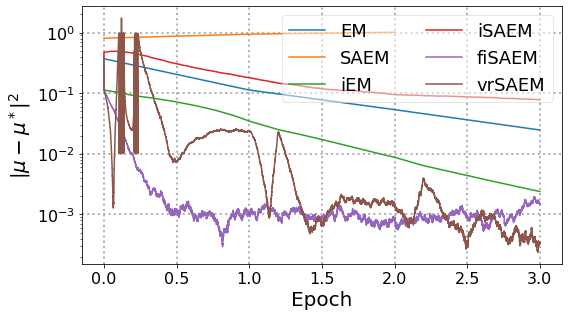
\includegraphics[width=\textwidth]{pic_paper/gmm_tts.png}\vspace{-.2cm}
\caption{TO COMPLETE}\vspace{-.2cm}
\label{fig:gmm_tts}
\end{figure}

\end{minipage}
\end{wrapfigure}

The number of MC samples is fixed to $M=40$ chains.
Figure \ref{fig:gmm_tts} shows the convergence of the precision $|\mu - \mu^*|^2$ for the different methods against the epoch(s) elapsed (one epoch equals $n$ iterations). We observe that the \SAEMVR\ and \FISAEM\ methods outperform the other methods, supporting our analytical results.




\subsection{Deformable Template Model for Image Analysis}
We now run our different methods using an example taken from \citep{allassonniere2010construction}.
Let $(y_i, i \in \inter)$ be observed images. 
Let $u \in \mathcal{U} \subset \rset^2$ denote the pixel index on the image and $x_u \in \mathcal{D} \subset \rset^2$ its location.

The model used in this experiment suggests that each image $y_i$ is a deformation of a template, noted $I: \mathcal{D} \to \rset$, common to all images of the dataset:
\beq\label{eq:deformablemodel}
y_{i}(u)=I\left(x_{u}-\Phi_{i}\left(x_{u}\right)\right)+\varepsilon_{i}(u)
\eeq
where $\phi_i: \rset^2 \to \rset^2$ is a deformation function, and $\varepsilon_{i} \sim \mathcal{N}(0,\sigma^2)$ is an observation error.

The template model, given $(p_k, k \in \llbracket 1, k_p \rrbracket)$ landmarks on the template, a fixed known kernel $\mathbf{K}_{\mathbf{p}}$ and a vector of parameters $\beta \in \rset^{k_p}$ is defined as follows:
\beq
I_{\xi}=\mathbf{K}_{\mathbf{p}} \beta, \quad \textrm{where} \quad \left(\mathbf{K}_{\mathbf{p}} \beta \right)(x)=\sum_{k=1}^{k_{p}} \mathbf{K}_{\mathbf{p}}\left(x, p_{k}\right) \beta_k
\eeq

Besides, we parameterize the deformation model given some landmarks $(g_k, k \in \llbracket 1, k_g \rrbracket)$ and a fixed kernel $\mathbf{K}_{\mathbf{g}}$ as:
\beq
\Phi_{i}(x)=\left(\mathbf{K}_{\mathbf{g}} z_{i}\right)(x)=\sum_{k=1}^{k_{s}} \mathbf{K}_{\mathbf{g}}\left(x, g_{k}\right)\left(z_{i}^{(1)}(k), z_{i}^{(2)}(k)\right)
\eeq
where $z_i \sim \mathcal(0,\Gamma)$ and $z_i \in \left( \rset^{k_g}\right)^2$.



\section{Conclusion}


\newpage
\linespread{1.1}
\normalsize

\bibliographystyle{abbrvnat}
\bibliography{references}

\linespread{1}
\newpage

\appendix


\section{Proof of Lemma~\ref{lem:growth}}\label{app:growth}
\begin{Lemma*} 
Assume H\ref{ass:reg},H\ref{ass:eigen}. For all $\bss \in \Sset$,
\beq \label{eq:semigrad}
\upsilon_{\min}^{-1} \pscal{\grd V ( {\bss} ) }{ {\bss} - \os( \op ({\bss})) }
\geq \big\| {\bss} - \os( \op ({\bss})) \big\|^2 \geq \upsilon_{\max}^{-2} \| \grd V ( {\bss} ) \|^2,
\eeq
\end{Lemma*}
\begin{proof}
Using H\ref{ass:reg} and the fact that we can exchange integration with differentiation and the Fisher's identity,   we obtain
\beq \label{eq:grd_v}
\begin{split}
\grd_{ \bss} V( {\bss} ) & = \jacob{ \overline{\param} }{ \bss }{\bss}^\top
\Big( \grd_\param \Pen( \mstep{\bss} )  + \grd_\param \calL( \overline\param( {\bss} ) )  \Big) \\
& =  \jacob{ \overline{\param} }{ \bss }{\bss}^\top \Big( \grd_\param \psi( \mstep{\bss}) + \grd_\param \Pen( \mstep{\bss} ) - \jacob{\phi}{\param}{\mstep{\bss} }^\top  \os( \op ({\bss})) \Big)\\
& =   \jacob{ \overline{\param} }{ \bss }{\bss}^\top \jacob{\phi}{\param}{ \mstep{\bss} }^\top \!~ ({\bss} - \os( \op ({\bss})) ) \eqsp,
\end{split}
\eeq
Consider the following vector map:
\beq
{\bss} \to \grd_{\param} L(\bss, \param) \vert_{\param= \mstep{\bss}}= \grd_\param \psi ( \mstep{\bss} ) + \grd_{ \param} \Pen(\mstep{\bss}  ) - \jacob{ \phi }{ \param }{\mstep{\bss}  }^\top \!~{\bss} \eqsp.
\eeq
Taking the gradient of the above map \wrt ${\bss}$ and using assumption H\ref{ass:reg}, we show that:
\beq
{\bm 0} = - \jacob{\phi}{\param}{\mstep{\bss} } + \Big( \underbrace{ \grd_{\param}^2 \big( \psi( \param ) + \Pen( \param ) - \pscal{ \phi( \param ) }{ {\bss} } \big)}_{= \hess{{L}}{\param} ( {\bss}; \param )} \big|_{\param = \mstep{\bss}  } \Big) \jacob{ \overline{\param} }{\bss}{\bss} \eqsp.
\eeq
The above yields
\beq
\grd_{ \bss} V( {\bss} )  = \operatorname{B}(\bss) ({\bss} - \os( \op ({\bss})) )
\eeq
where we recall $\operatorname{B}(\bss) = \jacob{ \phi }{ \param }{ \mstep{\bss} } \Big( \hess{{L}}{\param}( {\bss}; \mstep{\bss} )  \Big)^{-1} \jacob{ \phi }{ \param }{\mstep{\bss} }^\top$. The proof of \eqref{eq:semigrad} follows directly from the assumption~H\ref{ass:eigen}.
\end{proof}


\section{Proof of Lemma~\ref{lem:meanfield_isaem}}
\begin{Lemma*}
 Assume H\ref{ass:convset}. The update \eqref{eq:isaem} is equivalent to the following update on the resulting statistics 
\beq
\hat{\bss}^{(k+1)} =  \hat{\bss}^{(k)}  + \gamma_{k+1} \big( \tilde{S}^{(k+1)} - \hat{\bss}^{(k)} \big)
\eeq 
Also:
\beq
\EE\left[\tilde{S}^{(k+1)} - \hat{\bss}^{(k)}\right] = \EE\left[\overline{\bss}^{(k)} - \hat{\bss}^{(k)}\right] + \left(1 - \frac{1}{n} \right) \EE\left[\frac{1}{n} \sum_{i=1}^n \tilde{S}_i^{(\tau_i^k)}- \hat{\bss}^{(k)}\right]  +\frac{1}{n}\EE\left[\eta_{i_k}^{(k+1)}\right]
\eeq
where $\overline{\bss}^{(k)}$ is defined by \eqref{eq:definition-overline-bss} and $\tau_i^k = \max \{ k' : i_{k'} = i,~k' < k \}$.
\end{Lemma*}
\begin{proof}
From update \eqref{eq:isaem}, we have:
\beq
\begin{split}
\tilde{S}^{(k+1)} - \hat{\bss}^{(k)} & = \tilde{S}^{(k)} - \hat{\bss}^{(k)} +\frac{1}{n}\left( \tilde{S}_{i_k}^{(k+1)} - \tilde{S}_{i_k}^{(\tau_i^k)}  \right)\\
& = \overline{\bss}^{(k)} - \hat{\bss}^{(k)} + \tilde{S}^{(k)}- \overline{\bss}^{(k)}  - \frac{1}{n}\left( \tilde{S}_{i_k}^{(\tau_i^k)} - \tilde{S}_{i_k}^{(k+1)}   \right)
\end{split}
\eeq
Since $\tilde{S}_{i_k}^{(k+1)} = \overline{\bss}_{i_k}(\param^{(k)}) + \eta_{i_k}^{(k+1)}$ we have 
\beq
\begin{split}
\tilde{S}^{(k+1)} - \hat{\bss}^{(k)} = \overline{\bss}^{(k)} - \hat{\bss}^{(k)} + \tilde{S}^{(k)}- \overline{\bss}^{(k)}  - \frac{1}{n}\left( \tilde{S}_{i_k}^{(\tau_i^k)} -  \overline{\bss}_{i_k}(\param^{(k)})   \right) - \frac{1}{n}\eta_{i_k}^{(k+1)}
\end{split}
\eeq
Taking the full expectation of both side of the equation leads to:
\beq
\begin{split}
\EE\left[\tilde{S}^{(k+1)} - \hat{\bss}^{(k)}\right] = \EE\left[\overline{\bss}^{(k)} - \hat{\bss}^{(k)}\right] & + \EE\left[\frac{1}{n} \sum_{i=1}^n \tilde{S}_i^{(\tau_i^k)}-  \overline{\bss}^{(k)}\right] \\
& -\frac{1}{n} \EE\left[\EE\left[ \tilde{S}_i^{(\tau_i^k)}-  \overline{\bss}_{i_k}(\param^{(k)})  | \mathcal{F}_{k} \right]\right] - \frac{1}{n} \EE\left[\eta_{i_k}^{(k+1)}\right]
\end{split}
\eeq
The following equalities:
\beq
\EE\left[ \tilde{S}_i^{(\tau_i^k)} | \mathcal{F}_{k} \right] =\frac{1}{n} \sum_{i=1}^n \tilde{S}_i^{(\tau_i^k)} \quad \textrm{and} \quad \EE\left[  \overline{\bss}_{i_k}(\param^{(k)})  | \mathcal{F}_{k} \right]= \overline{\bss}^{(k)}
\eeq 
concludes the proof of the Lemma.
\end{proof}
 

\section{Proof of Theorem~\ref{thm:isaem}}\label{app:theoremisaem}
\begin{Theorem*}
Let $K_{\max }$ be a positive integer. 
Let $\left\{\gamma_{k}, k \in \mathbb{N}\right\}$ be a sequence of positive step sizes and consider the \ISAEM\ sequence $\left\{\hat{\bss}^{(k)}, k \in \mathbb{N}\right\}$ obtained with $\rho_{k+1}=1$ for any $k>0$.

Assume that $ \hat{\bss}^{(k)} \in \mathcal{S}$ for any $k \leq K_{\max }$.

\textcolor{red}{TO COMPLETE WITH BOUND}

\end{Theorem*} 

\begin{proof}

We begin our proof by giving this auxiliary Lemma setting an upper bound for the quantity $\EE[ \|  \hs{k} - \tilde{S}^{(k+1)}  \|^2 ]$
\begin{Lemma}\label{lem:aux2}
For any $k \geq 0$ and consider the \ISAEM\ update in \eqref{eq:isaem}, it holds that
\beq
\begin{split}
\EE \left[ \|  \tilde{S}^{(k+1)} - \hs{k}   \|^2 \right] \leq &4 \EE\left[ \|  \os^{(k)} - \hs{k} \|^2 \right] 
+ \frac{2\Lip{\bss}}{n^3} \sum_{i=1}^n \EE\left[ \| \hs{k} - \hs{t_i^k} \|^2 \right]\\
&+ 2\frac{C_{\eta}}{M_k} + 4 \EE\left[\norm{ \frac{1}{n} \sum_{i=1}^n \tilde{S}_i^{(\tau_i^k)}-  \overline{\bss}^{(k)}}^2\right] 
\end{split}
\eeq
\end{Lemma}

\begin{proof}
Applying the \ISAEM\ update yields:
\beq
\begin{split}
 \EE[ \|  \tilde{S}^{(k+1)} - \hs{k} \|^2 ] &=  \EE[ \| \tilde{S}^{(k)} - \hs{k}  -\frac{1}{n}\big(\tilde{S}^{(\tau_i^k)}_{i_k} - \tilde{S}^{(k)}_{i_k}  \big)  \|^2 ]\\
 & \leq  4 \EE\left[\norm{ \frac{1}{n} \sum_{i=1}^n \tilde{S}_i^{(\tau_i^k)}-  \overline{\bss}^{(k)}}^2\right] + 4 \EE\left[\norm{   \overline{\bss}^{(k)} - \hs{k} }^2\right] \\
 &+  \frac{2}{n^2} \EE\big[ \norm{ \os_{i_k}^{(k)} - \os_{i_k}^{(t_{i_k}^k)} }^2\big] + 2\frac{C_{\eta}}{M_k}
\end{split}
\eeq

The last expectation can be further bounded by
\beq
\begin{split}
&
\frac{2}{n^2}\EE[ \| \os_{i_k}^{(k)} - \os_{i_k}^{(t_{i_k}^k)} \|^2 ] = \frac{2}{n^3} \sum_{i=1}^n \EE[ \| \os_i^{(k)} - \os_i^{(t_i^k)} \|^2 ] \overset{(a)}{\leq} \frac{2\Lip{\bss}}{n^3}
\sum_{i=1}^n \EE[ \| \hs{k} - \hs{t_i^k} \|^2 ],
\end{split}
\eeq
where (a) is due to Lemma~\ref{lem:smooth} and which concludes the proof of the Lemma.

\end{proof}


Under the smoothness of the Lyapunov function $V$ (cf. Lemma~\ref{lem:smooth}), we can write:
\beq
\begin{split}
V( \hs{k+1} ) & \leq V( \hs{k} ) + \gamma_{k+1} \pscal{  \tilde{S}^{(k+1)}  - \hs{k}}{ \grd V( \hs{k} ) } + \frac{\gamma_{k+1}^2 \Lip{V}}{2} \|\tilde{S}^{(k+1)} -  \hs{k}  \|^2 \\
\end{split}
\eeq

Taking the expectation on both sidesyields:
\beq
\EE \left[V( \hs{k+1} ) \right]  \leq \EE \left[ V( \hs{k} ) \right] + \gamma_{k+1} \EE \left[\pscal{  \tilde{S}^{(k+1)}  - \hs{k}}{ \grd V( \hs{k} ) }  \right]+ \frac{\gamma_{k+1}^2 \Lip{V}}{2} \EE \left[\|\tilde{S}^{(k+1)} -  \hs{k}  \|^2  \right]
\eeq

Using Lemma~\ref{lem:meanfield_isaem}, we obtain:
\beq
\begin{split}
\EE \left[\pscal{  \tilde{S}^{(k+1)}  - \hs{k}}{ \grd V( \hs{k} ) }  \right] = & \EE \left[\pscal{  \overline{\bss}^{(k)}  - \hs{k}}{ \grd V( \hs{k} ) }  \right]  + \left(1 - \frac{1}{n}\right)\EE\left[\pscal{ \frac{1}{n} \sum_{i=1}^n \tilde{S}_i^{(\tau_i^k)}-  \overline{\bss}^{(k)}}{ \grd V( \hs{k} ) }\right] \\
& +  \frac{1}{n} \EE \left[\pscal{ \eta_{i_k}^{(k)}}{ \grd V( \hs{k} ) }  \right]\\
& \overset{(a)}{\leq} -\upsilon_{\min}\EE \left[\norm{  \overline{\bss}^{(k)}  - \hs{k}}^2  \right] + \left(1 - \frac{1}{n}\right)\EE\left[\pscal{ \frac{1}{n} \sum_{i=1}^n \tilde{S}_i^{(\tau_i^k)}-  \overline{\bss}^{(k)}}{ \grd V( \hs{k} ) }\right] \\
& +  \frac{1}{n} \EE \left[\pscal{ \eta_{i_k}^{(k)}}{ \grd V( \hs{k} ) }  \right]\\
& \overset{(b)}{\leq} -\upsilon_{\min}\EE \left[\norm{  \overline{\bss}^{(k)}  - \hs{k}}^2  \right] + \frac{1 - \frac{1}{n}}{2\beta}\EE\left[\norm{ \frac{1}{n} \sum_{i=1}^n \tilde{S}_i^{(\tau_i^k)}-  \overline{\bss}^{(k)}}^2\right]\\
& + \frac{\beta(n-1) + 1}{2n}\EE\left[ \norm{\grd V( \hs{k} )}^2\right]  +  \frac{1}{2 n} \EE \left[\norm{ \eta_{i_k}^{(k)}}^2 \right] \\
& \overset{(a)}{\leq} \left(\upsilon^2_{\max}\frac{\beta(n-1) + 1}{2n}-\upsilon_{\min}\right) \EE \left[\norm{  \overline{\bss}^{(k)}  - \hs{k}}^2  \right] \\
& + \frac{1 - \frac{1}{n}}{2\beta}\EE\left[\norm{ \frac{1}{n} \sum_{i=1}^n \tilde{S}_i^{(\tau_i^k)}-  \overline{\bss}^{(k)}}^2\right]+  \frac{1}{2 n} \EE \left[\norm{ \eta_{i_k}^{(k)}}^2 \right] 
\end{split}
\eeq
where (a) is due to the growth condition \eqref{lem:growth} and (b) is due to Young's inequality (with $\beta \to 1$).
Note $a_k = \gamma_{k+1}\left(\upsilon_{\min} - \upsilon^2_{\max}\frac{\beta(n-1) + 1}{2n}\right) $ and
\beq\label{eq:final1}
\begin{split}
a_k \EE \left[\norm{  \overline{\bss}^{(k)}  - \hs{k}}^2  \right]  \leq & \EE \left[ V( \hs{k} ) - V( \hs{k+1} ) \right] + \frac{\gamma_{k+1}^2 \Lip{V}}{2} \EE \left[\|\tilde{S}^{(k+1)} -  \hs{k}  \|^2  \right]\\
&+ \frac{\gamma_{k+1}(1 - \frac{1}{n})}{2\beta}\EE\left[\norm{ \frac{1}{n} \sum_{i=1}^n \tilde{S}_i^{(\tau_i^k)}-  \overline{\bss}^{(k)}}^2\right]+  \frac{\gamma_{k+1}}{2 n} \EE \left[\norm{ \eta_{i_k}^{(k)}}^2 \right] 
\end{split}
\eeq

We now give an upper bound of $\EE \left[\|\tilde{S}^{(k+1)} -  \hs{k}  \|^2  \right]$ using Lemma~\ref{lem:aux2} and plug it into \eqref{eq:final1}:

\beq\label{eq:final2}
\begin{split}
\left( a_k - 2\gamma_{k+1}^2 \Lip{V} \right) \EE \left[\norm{  \overline{\bss}^{(k)}  - \hs{k}}^2  \right]  \leq &  \EE \left[ V( \hs{k} ) - V( \hs{k+1} ) \right] \\
&  \frac{\gamma_{k+1}^3 \Lip{V}(1 - \frac{1}{n})}{\beta}\EE\left[\norm{ \frac{1}{n} \sum_{i=1}^n \tilde{S}_i^{(\tau_i^k)}-  \overline{\bss}^{(k)}}^2\right]\\
& +  \frac{\gamma_{k+1}}{2 n} \EE \left[\norm{ \eta_{i_k}^{(k)}}^2 \right] \\
& + \frac{\gamma_{k+1}^2 \Lip{V}\Lip{\bss}}{2 n^4} \sum_{i=1}^n \EE[ \| \hs{k} - \hs{t_i^k} \|^2 ]
\end{split}
\eeq



When, for any $k >0$, $\alpha_k > 0$, we have by Lemma~\ref{lem:growth} that:
\beq
\sum_{k=0}^{K_{\max}} \alpha_k \EE \left[\norm{\grd V( \hs{k} )}^2 \right] \leq \upsilon_{\max}^2\sum_{k=0}^{K_{\max}} \alpha_k \EE \left[\norm{  \overline{\bss}^{(k)}  - \hs{k}}^2  \right] 
\eeq
which yields an upper bound of the gradient of the Lyapunov function $V$ along the path of the \ISAEM\ update and concludes the proof of the Theorem.
\end{proof}



\clearpage

\section{Proof of Theorem~\ref{thm:fisaem}}\label{app:theoremfisaem}
\begin{Theorem*}
Let $K_{\max }$ be a positive integer. 
Let $\left\{\gamma_{k}, k \in \mathbb{N}\right\}$ be a sequence of positive step sizes and consider the \FISAEM\ sequence $\left\{\hat{\bss}^{(k)}, k \in \mathbb{N}\right\}$ obtained with $\rho_{k+1}=1$ for any $k>0$.

Assume that $ \hat{\bss}^{(k)} \in \mathcal{S}$ for any $k \leq K_{\max }$.

\textcolor{red}{TO COMPLETE WITH BOUND}

\end{Theorem*} 

\begin{proof}
We begin our proof by giving this auxiliary Lemma setting an upper bound for the quantity $\EE[ \|  \hs{k} - \tilde{S}^{(k+1)}  \|^2 ]$
\begin{Lemma}\label{lem:aux1}
For any $k \geq 0$ and consider the \FISAEM\ update in \eqref{eq:fisaem} with $\rho_k = \rho$, it holds that
\beq
\begin{split}
\EE[ \|  \hs{k} - \tilde{S}^{(k+1)}  \|^2 ] \leq &4 \rho^2 \EE[ \| \hs{k} - \os^{(k)} \|^2 ] + \frac{4\rho^2 \Lip{\bss}^2}{n} \sum_{i=1}^n  \EE[ \|  \hs{k} -\hs{t_i^k}  \|^2 ]\\
& + 2 \rho^2  \frac{C_{\eta}}{M_k} + 4 (1-\rho)^2 \EE[ \|  \hs{k} - \tilde{S}^{(k)}  \|^2 ] 
\end{split}
\eeq
\end{Lemma}
\begin{proof}
Applying the \FISAEM\ update yields:
\beq
\begin{split}
& \EE[ \| \hs{k} -  \tilde{S}^{(k+1)} \|^2 ] = \EE[ \| \hs{k} -  \tilde{S}^{(k)} +  \rho (\tilde{S}^{(k)} -\StocEstep^{(k+1)} ) \|^2 ] \\
& =  \EE[ \| (1-\rho)( \hs{k} -  \tilde{S}^{(k)}) +\rho(\hs{k} -\overline{\bss}^{(k)} ) +  \rho \left[ (\overline{\bss}^{(k)} -\overline{\StocEstep}^{(k)}) - ( \tilde{S}_{i_k}^{(k)}) - \tilde{S}_{i_k}^{(\tau_i^k)} \right] \|^2 ]
\end{split}
\eeq
We observe that $ \overline{\StocEstep}^{(k)} = \frac{1}{n} \sum_{i=1}^n \os_i^{(t_i^k)}$ and $\EE[ \tilde{S}_{i_k}^{(k)}) - \tilde{S}_{i_k}^{(\tau_i^k)} ] = \overline{\bss}^{(k)} -\overline{\StocEstep}^{(k)} + \EE[\eta_{i_k}^{(\tau_i^k)}]$. Thus
\beq
\begin{split}
& \EE[ \| \hs{k} -  \tilde{S}^{(k+1)} \|^2 ]\\
& \leq  4(1-\rho)^2 \EE\big[ \|  \hs{k} -  \tilde{S}^{(k)} \|^2 \big]  + 4\rho^2 \EE\big[ \| \hs{k} -\overline{\bss}^{(k)}  \|^2 \big] + 2\rho^2 \EE\big[ \norm{ \os_{i_k}^{(k)} - \os_{i_k}^{(t_{i_k}^k)} }^2\big] + 2\rho^2\frac{C_{\eta}}{M_k}
\end{split}
\eeq
where we use the variance inequality.
The last expectation can be further bounded by
\beq
\begin{split}
&
\EE[ \| \os_{i_k}^{(k)} - \os_{i_k}^{(t_{i_k}^k)} \|^2 ] = \frac{1}{n} \sum_{i=1}^n \EE[ \| \os_i^{(k)} - \os_i^{(t_i^k)} \|^2 ] \overset{(a)}{\leq} \frac{\Lip{\bss}}{n}
\sum_{i=1}^n \EE[ \| \hs{k} - \hs{t_i^k} \|^2 ],
\end{split}
\eeq
where (a) is due to Lemma~\ref{lem:smooth} and which concludes the proof of the Lemma.

\end{proof}
Using the smoothness of $V$ and update \eqref{eq:fisaem}, we obtain:
\beq
\begin{split}
V( \hs{k+1} ) & \leq V( \hs{k} ) - \gamma_{k+1} \pscal{  \hs{k} -  \tilde{S}^{(k+1)} }{ \grd V( \hs{k} ) } + \frac{\gamma_{k+1}^2 \Lip{V}}{2} \|  \hs{k} -  \tilde{S}^{(k+1)}  \|^2 \\
&  \leq V( \hs{k} ) - \gamma_{k+1} \pscal{  \hs{k} -  \tilde{S}^{(k)} }{ \grd V( \hs{k} ) } \\
& - \gamma_{k+1}\rho \pscal{  \tilde{S}^{(k)}  - \StocEstep^{(k+1)} }{ \grd V( \hs{k} ) } + \frac{\gamma_{k+1}^2 \Lip{V}}{2} \|  \hs{k} -  \tilde{S}^{(k+1)}  \|^2 \\
&  \leq V( \hs{k} )- \gamma_{k+1}\rho \pscal{   \hs{k} - \StocEstep^{(k+1)} }{ \grd V( \hs{k} ) }  \\
& - \gamma_{k+1}(1-\rho) \pscal{  \hs{k} -  \tilde{S}^{(k)} }{ \grd V( \hs{k} ) } + \frac{\gamma_{k+1}^2 \Lip{V}}{2} \|  \hs{k} -  \tilde{S}^{(k+1)}  \|^2 
\end{split}
\eeq
Taking the expectaitons on both sides and noting that $\EE[ \StocEstep^{(k+1)} ] = \EE\left[ \EE[    \StocEstep^{(k+1)}  | \mathcal{F}_k] \right] = \os^{(k)}$ (independence of both indices $i_k$ and $j_k$) ,we have:
\beq
\begin{split}
\EE[V( \hs{k+1} ) - V( \hs{k} )] & \leq  - \gamma_{k+1}\rho \EE[\pscal{  \hs{k} -  \os^{(k)} }{ \grd V( \hs{k} ) } ] \\
& - \gamma_{k+1}(1-\rho) \EE[ \pscal{  \hs{k} -  \tilde{S}^{(k)} }{ \grd V( \hs{k} ) }]+ \frac{\gamma_{k+1}^2 \Lip{V}}{2} \EE[ \|  \hs{k} -  \tilde{S}^{(k+1)}  \|^2] \\
& \overset{(a)}{\leq} - (\gamma_{k+1} \upsilon_{\max}^2\frac{(1-\rho)}{2} + \gamma_{k+1}\rho) \EE\left[\norm{ \hs{k} -  \os^{(k)} }^2\right] -  \gamma_{k+1}\frac{1-\rho}{2 }\EE\big[\norm{ \hs{k} -  \tilde{S}^{(k)} }^2\big]\\
& + \frac{\gamma_{k+1}^2 \Lip{V}}{2} \EE[ \|  \hs{k} -  \tilde{S}^{(k+1)}  \|^2]  
\end{split}
\eeq
where $(a)$ used the growth condition \eqref{eq:semigrad} twice (on $\pscal{  \hs{k} -  \os^{(k)} }{ \grd V( \hs{k} ) } $ and $\norm{\grd V( \hs{k} }^2$ and the triangle inequality.

\paragraph{ Bounding $\EE[ \|  \hs{k} -  \tilde{S}^{(k+1)}  \|^2]  $} Using Lemma~\ref{lem:aux1}, we obtain:
\beq
\begin{split}
\EE[V( \hs{k+1} ) - V( \hs{k} )] \leq  & - \gamma_{k+1} \big(   \upsilon_{\max}^2\frac{(1-\rho)}{2} +  \rho  - 2\rho^2\gamma_{k+1}   \Lip{V}  \big) \EE\left[\norm{ \hs{k} -  \os^{(k)} }^2\right]\\
& + \frac{2 \gamma_{k+1}^2 \Lip{V} \rho^2 \Lip{\bss}^2}{n} \sum_{i=1}^n  \EE[ \|  \hs{k} -\hs{t_i^k}  \|^2 ]\\
& + \gamma_{k+1} (1-\rho)\big( 2 \gamma_{k+1}\Lip{V} (1-\rho) - \frac{1}{2}    \big) \EE\big[\norm{ \hs{k} -  \tilde{S}^{(k)} }^2\big]\\
&  +  \gamma_{k+1}^2 \rho^2 \Lip{V}   \frac{C_{\eta}}{M_k} 
\end{split}
\eeq


Next, we observe that
\beq
\frac{1}{n} \sum_{i=1}^n \EE[ \| \hs{k+1} - \hs{t_i^{k+1}} \|^2 ] = \frac{1}{n} \sum_{i=1}^n
\Big( \frac{1}{n} \EE[ \| \hs{k+1} - \hs{k} \|^2 ] + \frac{n-1}{n} \EE[ \| \hs{k+1} - \hs{t_i^k} \|^2 ]  \Big)
\eeq
where the equality holds as $i_k$ and $j_k$ are drawn independently. For any $\beta > 0$, it holds
\beq
\begin{split}
& \EE[ \| \hs{k+1} - \hs{t_i^k} \|^2 ] \\
& = \EE \Big[ \| \hs{k+1} - \hs{k} \|^2 + \| \hs{k} - \hs{t_i^k} \|^2 + 2 \pscal{\hs{k+1} - \hs{k}}{\hs{k}- \hs{t_i^k}} \Big] \\
& = \EE \Big[ \| \hs{k+1} - \hs{k} \|^2 + \| \hs{k} - \hs{t_i^k} \|^2 - 2 \gamma_{k+1} \pscal{\hs{k} - \os^{(k)} }{\hs{k}- \hs{t_i^k}} \Big] \\
& \leq  \EE \Big[ \| \hs{k+1} - \hs{k} \|^2 + \| \hs{k} - \hs{t_i^k} \|^2 +  \frac{\gamma_{k+1}}{\beta} \| \hs{k} - \os^{(k)} \|^2 + \gamma_{k+1} \beta \| \hs{k}- \hs{t_i^k} \|^2 \Big]
\end{split}
\eeq
where the last inequality is due to the Young's inequality. Subsequently, we have
\beq
\begin{split}
& \frac{1}{n} \sum_{i=1}^n \EE[ \| \hs{k+1} - \hs{t_i^{k+1}} \|^2 ] \\
& \leq \EE[  \| \hs{k+1} - \hs{k} \|^2 ] + \frac{n-1}{n^2} \sum_{i=1}^n \EE \Big[ (1+\gamma_{k+1} \beta) \|  \hs{k} - \hs{t_i^k} \|^2 + \frac{\gamma_{k+1}}{\beta} \| \hs{k} - \os^{(k)} \|^2 \Big]
\end{split}
\eeq
Observe that $\hs{k+1} - \hs{k} =  \gamma_{k+1} (\tilde{S}^{(k+1)} -  \hs{k} )$. Applying Lemma~\ref{lem:aux1} yields:
\beq
\begin{split}
 \frac{1}{n} \sum_{i=1}^n \EE[ \| \hs{k+1} - \hs{t_i^{k+1}} \|^2 ]  \leq & \left( 4 \rho^2 +  \frac{\gamma_{k+1}}{\beta} \right) \EE[ \| \hs{k} - \os^{(k)} \|^2 ] \\
& +  \left(\frac{4\rho^2 \Lip{\bss}^2}{n} +  \frac{(n-1)(1+\gamma_{k+1} \beta)}{n^2}   \right) \sum_{i=1}^n  \EE[ \|  \hs{k} -\hs{t_i^k}  \|^2 ]\\
&  + 2 \rho^2  \frac{C_{\eta}}{M_k} + 4 (1-\rho)^2 \EE[ \|  \hs{k} - \tilde{S}^{(k)}  \|^2 ] 
\end{split}
\eeq
Define
\beq
\Delta^{(k)} \eqdef \frac{1}{n} \sum_{i=1}^n \EE[ \| \hs{k} - \hs{t_i^{k}} \|^2 ]
\eeq
and note that
\beq
\begin{split}
\Delta^{(k+1)} \leq  & \left(1-\frac{1}{n} + 4\rho^2 \Lip{\bss}^2 + \gamma_{k+1} \beta   \right)  \Delta^{(k)} +  \left( 4 \rho^2 +  \frac{\gamma_{k+1}}{\beta} \right) \EE[  \| \hs{k} - \os^{(k)} \|^2 ]\\
& + 2 \rho^2  \frac{C_{\eta}}{M_k} + 4 (1-\rho)^2 \EE[ \|  \hs{k} - \tilde{S}^{(k)}  \|^2 ] 
\end{split}
\eeq


\paragraph{ Bounding $ \EE\big[\norm{ \hs{k} -  \tilde{S}^{(k)} }^2\big] $} Remark that this term is the price we pay for the two time scale dynamics and corresponds to the gap between the two asynchronous updates (one is on  $\hs{k}$ and the other on $ \tilde{S}^{(k)}$).

\textcolor{red}{FIND AN UPPER BOUND TO THAT GAP}

%
%\beq\label{eq:rmstep}
%\textsf{SA-step}:~ \hat{\bss}^{(k+1)} =  \hat{\bss}^{(k)}  + \gamma_{k+1}(\tilde{S}^{(k+1)} - \hat{\bss}^{(k)} )
%\eeq
%\beq \label{eq:sestep}
%\textsf{Inexact-step}:~\tilde{S}^{(k+1)} = \tilde{S}^{(k)} + \rho_{k+1} \big( \StocEstep^{(k+1)}- \tilde{S}^{(k)}  \big),
%\eeq
%\begin{align}
%&\emph{(\ISAEM\ \citep{karimi2019non, kuhn2019properties})} & \StocEstep^{(k+1)} &= \StocEstep^{(k)} + {\textstyle \frac{1}{n}}\big( \tilde{S}_{i_k}^{(k)}  - \tilde{S}_{i_k}^{(\tau_{i_k}^k)} \big) \label{eq:isaem} \\
%&\emph{(\SAEMVR\ This paper )} &\StocEstep^{(k+1)} &= \tilde{S}^{(\ell(k))} +  \big( \tilde{S}_{i_k}^{(k)}  -\tilde{S}_{i_k}^{(\ell(k))}   \big) \label{eq:vrsaem}\\
%&\emph{(\FISAEM\ This paper )} &\StocEstep^{(k+1)} &= \overline{\StocEstep}^{(k)} + \big( \tilde{S}_{i_k}^{(k)}  - \tilde{S}_{i_k}^{(t_{i_k}^k)} \big) \label{eq:fisaem}\\
%&    &\overline{\StocEstep}^{(k+1)} &= \overline{\StocEstep}^{(k)} + n^{-1} \big( \tilde{S}_{j_k}^{(k)}  - \tilde{S}_{j_k}^{(t_{j_k}^k)} \big).
%%\emph{(SAGA-EM)} & ~~~~\StocEstep^{(k+1)} = s & \gamma_{k+1} =
%\end{align}

\end{proof}

\end{document}
